\section{Design and Application of a Metamaterial Superstrate on a Bio-Inspired Antenna for Partial Discharge Detection through Dielectric Windows}

\subsection*{Contexto y objetivo}
El monitoreo continuo de las descargas parciales (DP) en equipos de alta tensión es crucial para prevenir la degradación del aislamiento y fallas del equipo. El método tradicional IEC 60270 es invasivo. El método radiométrico o de Ultra Alta Frecuencia (UHF) es una alternativa no invasiva, detectando ondas electromagnéticas emitidas por las DP en el rango de 300 MHz a 3 GHz. Las antenas monopolo impresas (PMA) son adecuadas para esto debido a su bajo costo, patrones de radiación atractivos, amplio ancho de banda y facilidad de construcción, pero las PMA tradicionales suelen ser grandes y requieren una alta ganancia para detectar DP de baja intensidad.

Este trabajo se basa en una PMA bioinspirada (basada en la hoja de \textit{Jatropha mollissima}) desarrollada previamente, que ya cumple con los requisitos de tamaño, ancho de banda y ganancia para la detección de DP a través de ventanas dieléctricas. El objetivo principal de este estudio es diseñar un superestrato de metamaterial, utilizando ventanas dieléctricas existentes, para mejorar la sensibilidad de detección de DP de esta PMA bioinspirada. Se busca mejorar específicamente la ganancia, el ancho de banda y el patrón de radiación de la antena mediante la incorporación de resonadores de anillo dividido (SRR) y tiras de carga capacitivas (CLS) en el superestrato dieléctrico.

\subsection*{Metodología o desarrollo}
La metodología se dividió en tres etapas: procedimientos computacionales, pruebas experimentales de laboratorio y aplicación en campo.

\subsubsection*{Procedimientos Computacionales}
Se utilizó el software HFSS (High Frequency Structure Simulator) para el diseño y simulación. El sustrato empleado fue FR-4 con $\varepsilon_r = 4.4$, un espesor $h = 1.6$ mm y una tangente de pérdidas $\delta = 0.02$. Las simulaciones se realizaron en un rango de frecuencia de 200 MHz a 1600 MHz.

\begin{itemize}
    \item \textbf{Diseño de la PMA Bioinspirada}: Se utilizó una estructura basada en la hoja de \textit{Jatropha mollissima} (Pohl) Baill, cuyas dimensiones finales se muestran en la Figura \ref{fig:PMA_design}.
    \begin{figure}[htpb]
    \centering
    
\includegraphics[width=0.8\textwidth]{images/f1c5b012cd86bd42b78fd9b9b77f9e22_p7_i2.png}
    \caption{PMA bioinspirada: detalles del modelo final diseñado (todas las dimensiones en centímetros) \cite{26}.}
    \end{figure}
    \item \textbf{Simulaciones de Celdas Unitarias de Metamaterial}: Se diseñaron y evaluaron estructuras SRR-CLS rectangulares y circulares para exhibir propiedades de doble negatividad (DNG) en el rango de frecuencia de actividad de DP (300--1500 MHz). Las dimensiones de estas celdas unitarias se presentan en la Figura \ref{fig:SRR_cells}.
    \begin{figure}[htpb]
    \centering
    
\includegraphics[width=0.8\textwidth]{images/f1c5b012cd86bd42b78fd9b9b77f9e22_p8_i1.jpeg}
    \caption{Modelos SRR para cada celda unitaria de metamaterial (las tiras verdes son las estructuras CLS): (a) rectangular.}
    \end{figure}
    Para la caracterización como metamateriales, cada modelo se simuló individualmente bajo condiciones de contorno específicas (paredes de conductor eléctrico perfecto (PEC) y de conductor magnético perfecto (PMC)), excitado por dos puertos de onda (Waveports), como se ilustra en la Figura \ref{fig:boundary_conditions}. Esto permitió la obtención de los coeficientes $S_{11}$ y $S_{21}$ para calcular la permitividad ($\varepsilon$) y permeabilidad ($\mu$) efectivas.
    \begin{figure}[htpb]
    \centering
    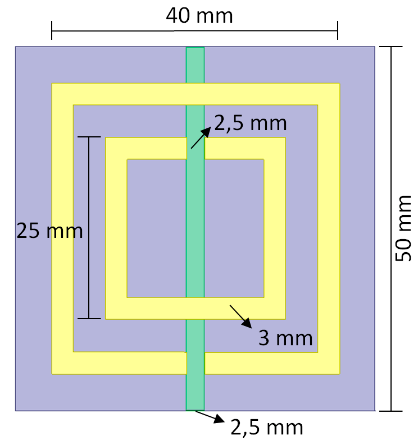
\includegraphics[width=0.8\textwidth]{images/f1c5b012cd86bd42b78fd9b9b77f9e22_p8_i3.png}
    \caption{Condiciones de contorno para los modelos SRR-CLS simulados.}
    \end{figure}
    \item \textbf{Simulaciones de Superestrato de Metamaterial}: Las celdas unitarias caracterizadas se posicionaron en una matriz de 3x3 como superestratos sobre la PMA bioinspirada, como se muestra en la Figura \ref{fig:superstrates}.
    \begin{figure}[htpb]
    \centering
    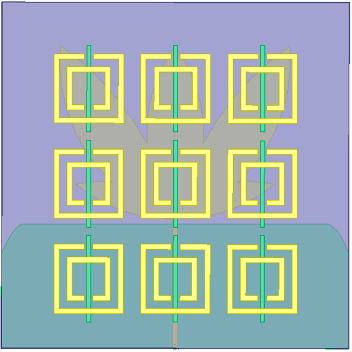
\includegraphics[width=0.8\textwidth]{images/f1c5b012cd86bd42b78fd9b9b77f9e22_p9_i1.png}
    \caption{Superestratos de metamaterial posicionados sobre la PMA bioinspirada: (a) rectangular.}
    \end{figure}
    La altura óptima del superestrato se definió en 135 mm para los SRR rectangulares y 125 mm para los circulares. Los espaciamientos entre celdas se ajustaron a 10x15 mm (rectangular) y 8x14 mm (circular), con una separación de 5 mm en las CLS. También se simuló la PMA solo con el material dieléctrico (FR-4) como superestrato para aislar el efecto del metamaterial.
\end{itemize}

\subsubsection*{Pruebas Experimentales de Laboratorio}
\begin{itemize}
    \item \textbf{Mediciones de Coeficiente de Reflexión y Ganancia}: Los valores del coeficiente de reflexión ($S_{11}$) se obtuvieron con un analizador de redes ENA E5062A. Las mediciones de ganancia se realizaron en una cámara anecoica con una antena de referencia (Hyperlog 30100X, 4.5 dBi de ganancia media) y la antena bajo prueba (AUT), como se esquematiza en la Figura \ref{fig:gain_setup}. La distancia al campo lejano (R) se estableció en 1.0 m. La ganancia de la antena bajo prueba ($G_D$) se calculó utilizando una ecuación de Friis adaptada.
    \begin{figure}[htpb]
    \centering
    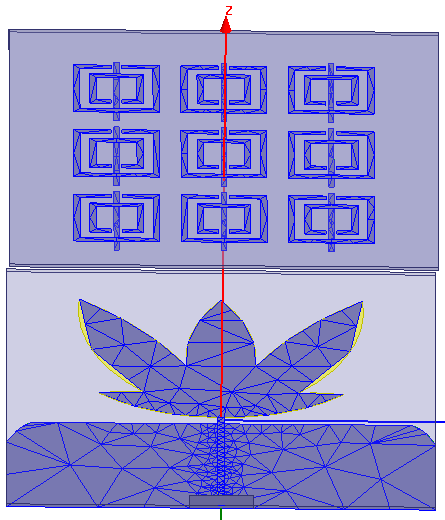
\includegraphics[width=0.8\textwidth]{images/f1c5b012cd86bd42b78fd9b9b77f9e22_p10_i1.png}
    \caption{Esquema de la configuración experimental utilizada en la prueba de medición de ganancia.}
    \end{figure}
    \item \textbf{Pruebas de Sensibilidad de Detección de DP}: Se utilizó una celda de aceite (configuración de electrodo punto-a-plano con disco de poliamida) como generador de DP, conectada a un capacitor de acoplamiento (1000 pF) y un circuito resonante (LDM-5). El montaje experimental se muestra en la Figura \ref{fig:PD_setup}. Las pulsos de DP se adquirieron con un osciloscopio Keysight DSO90604A. Se realizaron procedimientos de calibración según la norma IEC 60270 para correlacionar la carga aparente de DP con los valores de voltaje medidos.
    \begin{figure}[htpb]
    \centering
    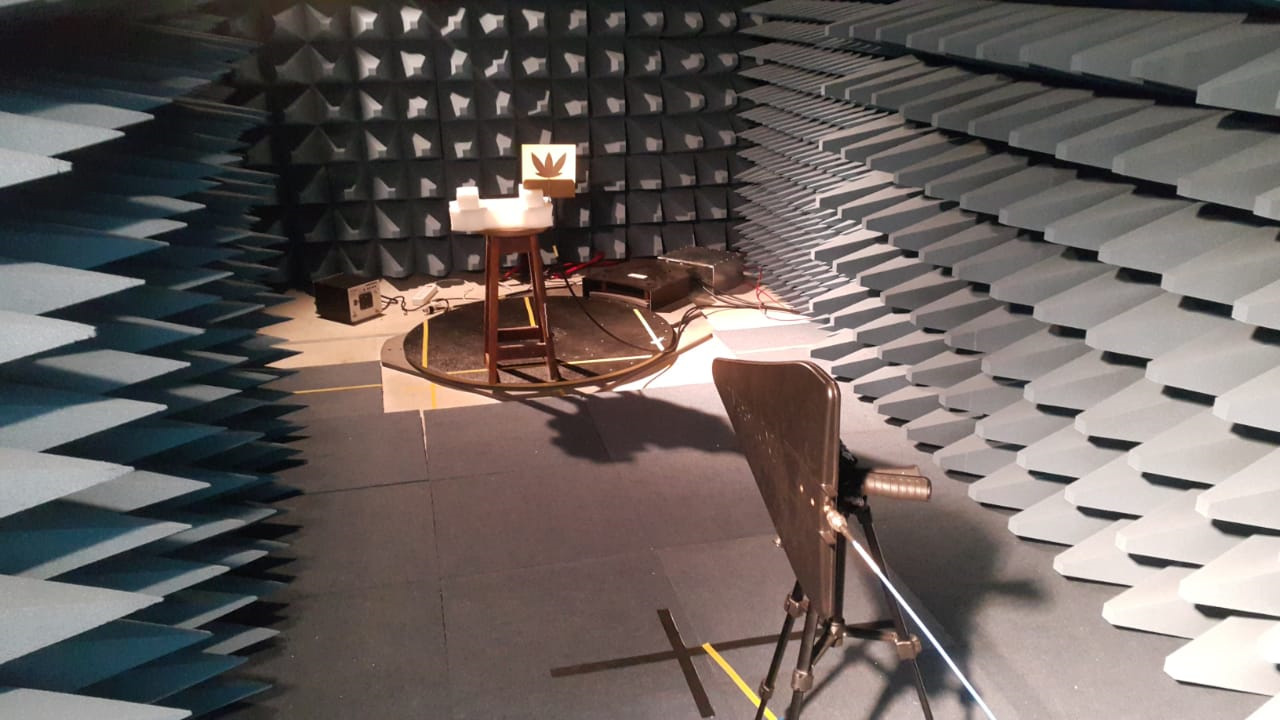
\includegraphics[width=0.8\textwidth]{images/f1c5b012cd86bd42b78fd9b9b77f9e22_p11_i1.jpeg}
    \caption{Configuración experimental aplicada para la medición de Descarga Parcial (PD).}
    \end{figure}
\end{itemize}

\subsubsection*{Aplicación en Campo}
El conjunto PMA-metamaterial se probó en un Transformador de Corriente (TC) de 230 kV en una subestación brasileña (Mussuré II). Este TC fue seleccionado por su degradación del aislamiento. Los pulsos de DP se adquirieron en el dominio del tiempo con un osciloscopio Tektronix TDS5104B. Para fines comparativos, la PMA bioinspirada sin superestrato también se utilizó simultáneamente a la misma distancia del TC. Un generador de señales se usó para producir una tensión de referencia sinusoidal y así identificar las señales de DP por su ubicación de fase y periodicidad. El TC se muestra en la Figura \ref{fig:CT_field}.
\begin{figure}[htpb]
\centering
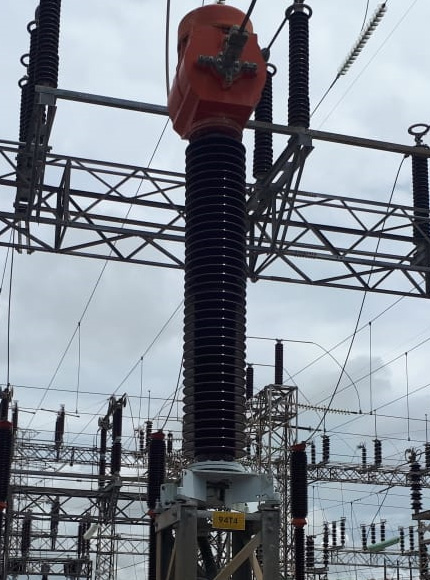
\includegraphics[width=0.8\textwidth]{images/f1c5b012cd86bd42b78fd9b9b77f9e22_p12_i1.jpeg}
\caption{El Transformador de Corriente de 230 kV evaluado en las pruebas de aplicación en campo.}
\end{figure}

\subsection*{Resultados o hallazgos}

\subsubsection*{Resultados de la Simulación}
\begin{itemize}
    \item \textbf{Ganancia de la PMA Bioinspirada}: La ganancia máxima simulada de la PMA bioinspirada mostró valores por debajo del umbral recomendado (2 dBi) para frecuencias cercanas a la frecuencia de operación inferior (487 MHz), como se observa en la Figura \ref{fig:PMA_gain_sim}.
    \begin{figure}[htpb]
    \centering
    \includegraphics[width=0.8\textwidth]{images/f1c5b012cd86bd42b78fd9b9b77f9e22_p13_i1.png}
    \caption{Ganancia máxima simulada de la PMA bioinspirada.}
    \end{figure}
    \item \textbf{Coeficientes de Reflexión de Celdas Unitarias de Metamaterial}: Las celdas unitarias circulares y rectangulares presentaron anchos de banda dentro del rango de actividad de DP, operando hasta 1033 MHz y 1117 MHz, respectivamente.
    \item \textbf{Valores de $\mu$ y $\varepsilon$ de Celdas Unitarias}: Ambas celdas unitarias de metamaterial exhibieron características de doble negatividad ($\varepsilon < 0$ y $\mu < 0$) en casi todo el rango de actividad de DP (300--1500 MHz), con la excepción de bandas específicas (1190--1350 MHz para SRR rectangular y 1100--1300 MHz para SRR circular) donde $\mu$ fue positiva. La Figura \ref{fig:meta_mu_eps} muestra un ejemplo para la celda circular.
    \begin{figure}[htpb]
    \centering
    \includegraphics[width=0.8\textwidth]{images/f1c5b012cd86bd42b78fd9b9b77f9e22_p14_i7.png}
    \caption{Valores de $\mu$ y $\varepsilon$ de celdas unitarias de metamaterial: (a) circular.}
    \end{figure}
    \item \textbf{Influencia del Superestrato en el Coeficiente de Reflexión}: La aplicación del superestrato (con o sin metamaterial) provocó desplazamientos en la frecuencia de operación inferior de la PMA. El superestrato de FR4 (sin metamaterial) mostró un desplazamiento de 42 MHz (reducción de ancho de banda del 5.2\%). Con el metamaterial, los desplazamientos fueron de 56 MHz (rectangular) y 77 MHz (circular). También hubo un aumento de la frecuencia superior (22 MHz para rectangular, 64 MHz para circular), resultando en una reducción total del ancho de banda del 3.9\% y 1.8\% respectivamente. Se observaron mejoras en los coeficientes de reflexión para el rango de 1050--1300 MHz (por debajo de -10 dB). La Figura \ref{fig:S11_comparison_sim} ilustra esta comparación.
    \begin{figure}[htpb]
    \centering
    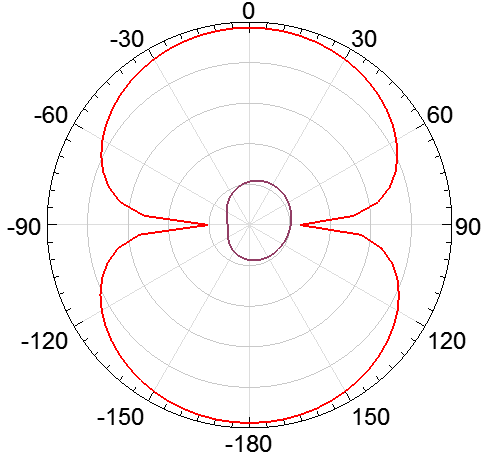
\includegraphics[width=0.8\textwidth]{images/f1c5b012cd86bd42b78fd9b9b77f9e22_p15_i1.png}
    \caption{Comparación entre los coeficientes de reflexión de las estructuras simuladas.}
    \end{figure}
    \item \textbf{Patrones de Radiación}: La adición del superestrato de FR4 no alteró significativamente los patrones de radiación de la PMA. Sin embargo, los superestratos SRR introdujeron distorsiones en los patrones de radiación en las frecuencias de operación superiores (Figuras 22-24 del documento original), siendo el SRR rectangular el que presentó menores distorsiones. Los patrones fueron adecuados para aplicaciones en ventanas dieléctricas, con la mayoría de los valores de radiación máxima concentrados en la dirección de acoplamiento (0°).
    \item \textbf{Ganancia Máxima}: La aplicación de ambos superestratos (SRR rectangular y circular) resultó en valores de ganancia máxima casi duplicados respecto a la PMA de referencia en el rango de 500--1000 MHz. El SRR circular también mostró una mejora significativa en el rango de 1300--1500 MHz. La ganancia fue superior a 2 dBi en todo el rango de 500--1500 MHz con la adición del metamaterial. La Figura \ref{fig:max_gain_comparison_sim} muestra la comparación. La ganancia media simulada para la PMA de referencia fue de 2.81 dBi, para el FR4 superestrato de 2.83 dBi, para el SRR rectangular de 3.96 dBi y para el SRR circular de 4.07 dBi. El SRR rectangular se seleccionó para las pruebas experimentales debido a su mejor relación ganancia/ancho de banda/patrón de radiación.
    \begin{figure}[htpb]
    \centering
    \includegraphics[width=0.8\textwidth]{images/f1c5b012cd86bd42b78fd9b9b77f9e22_p17_i4.png}
    \caption{Comparación entre los valores de ganancia máxima de las estructuras simuladas.}
    \end{figure}
\end{itemize}

\subsubsection*{Resultados Experimentales de Laboratorio}
\begin{itemize}
    \item \textbf{Antenas Fabricadas}: Se construyeron la PMA bioinspirada sin superestrato y con superestrato de metamaterial SRR rectangular, como se muestra en la Figura \ref{fig:PMA_manufactured}.
    \begin{figure}[htpb]
    \centering
    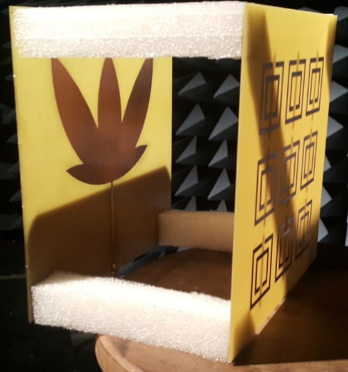
\includegraphics[width=0.8\textwidth]{images/f1c5b012cd86bd42b78fd9b9b77f9e22_p18_i2.jpeg}
    \caption{PMA bioinspirada fabricada: (b) con superestrato de metamaterial.}
    \end{figure}
    \item \textbf{Coeficientes de Reflexión Medidos}: Los resultados medidos y simulados mostraron un comportamiento similar. Para la PMA sin metamaterial, el ancho de banda medido fue de 472 MHz hasta valores superiores a 1500 MHz. Con el metamaterial, la frecuencia inferior se desplazó a 540 MHz (un desplazamiento de 68 MHz), y se verificó un mejor rendimiento del coeficiente de reflexión en el rango de 1.1–1.5 GHz. La Figura \ref{fig:S11_measured_sim} muestra la comparación.
    \begin{figure}[htpb]
    \centering
    \includegraphics[width=0.8\textwidth]{images/f1c5b012cd86bd42b78fd9b9b77f9e22_p18_i3.png}
    \caption{Coeficientes de reflexión medidos y simulados para la PMA bioinspirada con y sin superestrato de metamaterial.}
    \end{figure}
    \item \textbf{Ganancia Medida}: Las curvas de ganancia medidas y simuladas coincidieron en su comportamiento. La PMA sin metamaterial presentó una ganancia media medida de 2.92 dBi. Con el superestrato de metamaterial, la ganancia media medida fue de 3.61 dBi, lo que representa una mejora de 0.7 dBi. Esto resultó en una antena con valores de ganancia superiores a 2 dBi desde 575 MHz hasta 1.5 GHz, indicando una alta sensibilidad para la detección de DP. La Figura \ref{fig:gain_measured_sim} presenta la comparación.
    \begin{figure}[htpb]
    \centering
    \includegraphics[width=0.8\textwidth]{images/f1c5b012cd86bd42b78fd9b9b77f9e22_p19_i1.png}
    \caption{Ganancia medida y simulada para la PMA bioinspirada con y sin superestrato de metamaterial.}
    \end{figure}
    \item \textbf{Sensibilidad de Detección de DP}: El conjunto PMA-metamaterial detectó exitosamente todos los pulsos de DP generados en la celda de aceite (Figura \ref{fig:PD_pulses_lab}), que también fueron detectados por el método IEC 60270. Los voltajes medidos en los terminales de la antena fueron aproximadamente la mitad de los obtenidos por el método estándar. Las DP detectadas mostraron cargas aparentes entre 15 y 60 pC, un rango típico para DP de baja intensidad. Un espectrograma de los pulsos de DP (Figura \ref{fig:PD_spectrogram}) confirmó concentraciones de energía espectral hasta 1500 MHz, validando la cobertura del rango de frecuencia de interés (300--1500 MHz).
    \begin{figure}[htpb]
    \centering
    \includegraphics[width=0.8\textwidth]{images/f1c5b012cd86bd42b78fd9b9b77f9e22_p20_i1.png}
    \caption{Muestra de pulsos de DP detectados por el conjunto PMA-metamaterial bioinspirado y el método estándar IEC 60270, respectivamente, para la aplicación de 13.4 kV en la celda de aceite.}
    \end{figure}
    \begin{figure}[htpb]
    \centering
    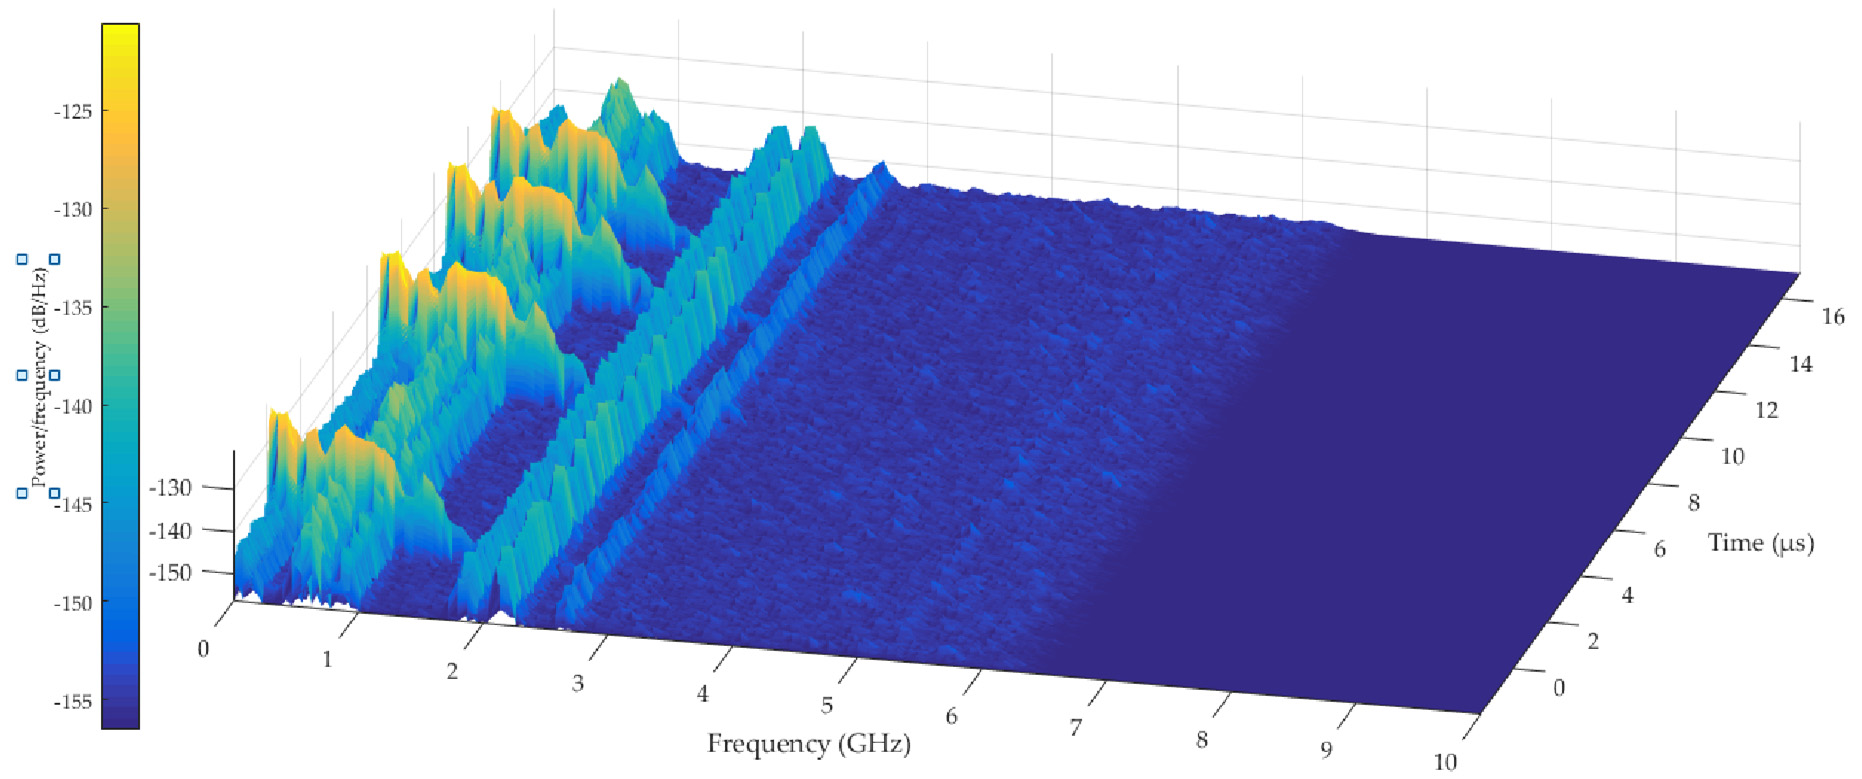
\includegraphics[width=0.8\textwidth]{images/f1c5b012cd86bd42b78fd9b9b77f9e22_p21_i1.jpeg}
    \caption{Espectrograma de la muestra de pulsos de DP detectada por el conjunto PMA-metamaterial bioinspirado presentado en la Figura \ref{fig:PD_pulses_lab}.}
    \end{figure}
\end{itemize}

\subsubsection*{Detección de DP en Subestación de 230 kV}
\begin{itemize}
    \item \textbf{Detección de DP}: El conjunto PMA-metamaterial detectó exitosamente señales con características de DP (transiciones de medio ciclo de tensión sinusoidal de referencia y desplazamiento de fase de aproximadamente 180° entre pulsos), como se muestra en la Figura \ref{fig:PD_pulses_field}. Presentó una mayor sensibilidad de detección, con amplitudes de señal casi duplicadas en comparación con la PMA de referencia sin superestrato.
    \begin{figure}[htpb]
    \centering
    \includegraphics[width=0.8\textwidth]{images/f1c5b012cd86bd42b78fd9b9b77f9e22_p21_i2.png}
    \caption{Comparación entre los pulsos de DP del Transformador de Corriente (TC) de 230 kV detectados por la PMA bioinspirada con y sin superestrato de metamaterial, respectivamente.}
    \end{figure}
    \item \textbf{Sensibilidad Práctica}: Se confirmó un nivel considerable de DP en el TC, lo que atestigua la sensibilidad práctica de la antena desarrollada para la detección de DP. No fue posible estimar los niveles de carga aparente de DP en campo debido a limitaciones prácticas.
\end{itemize}

\subsection*{Discusión o análisis crítico}
La integración del superestrato de metamaterial con la PMA bioinspirada ha demostrado ser una solución viable para mejorar la detección de DP. En comparación con antenas más competitivas como las Hornet o Vivaldi (Tabla 3 del documento original) que ofrecen mayor ganancia, el conjunto PMA-metamaterial presenta una ventaja significativa en sus dimensiones (200 mm $\times$ 200 mm $\times$ 135 mm) y facilidad de instalación en ventanas dieléctricas de equipos de alta tensión. Mientras que otras antenas de alta ganancia son considerablemente más grandes, el diseño propuesto logra una ganancia media de 3.61 dBi y un ancho de banda de 500--1500 MHz, características que son adecuadas para la detección de DP.

Aunque el método no permitió estimar la carga aparente de DP en las pruebas de campo, la capacidad de evaluar la evolución de la actividad de DP mediante la tensión inducida en los terminales de la antena es una valiosa información para el monitoreo continuo, no invasivo y de bajo costo. El trabajo futuro se centrará en técnicas de calibración, clasificación y localización para caracterizar completamente el sensor para diagnóstico de equipos de DP.

\subsection*{Conclusiones o implicaciones}
Las conclusiones principales de este estudio son:
\begin{enumerate}
    \item Ambas celdas unitarias SRR-CLS diseñadas mostraron un comportamiento de doble negatividad ($\mu < 0$, $\varepsilon < 0$) en casi todo el rango de frecuencia principal de actividad de DP (300--1500 MHz), clasificándolas como metamateriales aplicables como superestrato.
    \item La aplicación del superestrato de metamaterial resultó en desplazamientos en el rango de frecuencia de operación de la PMA, con reducciones de ancho de banda del 3.9\% para SRR rectangular y 1.8\% para SRR circular.
    \item A pesar de la reducción del ancho de banda, la aplicación de los superestratos de metamateriales resultó en valores de coeficiente de reflexión más altos para el rango de 1100--1500 MHz, mejorando la capacidad de transmisión/recepción de potencia de la antena.
    \item Se observaron distorsiones en los patrones de radiación en las frecuencias de operación superiores de la PMA para ambos superestratos de metamaterial, siendo el SRR rectangular el que presentó menores distorsiones, especialmente en la dirección del lóbulo posterior.
    \item La aplicación de ambos superestratos diseñados resultó en un aumento de la ganancia máxima casi al doble en el rango de frecuencia de 500--1000 MHz, con una mejora de la ganancia media superior a 1 dBi.
    \item La aplicación práctica del superestrato SRR rectangular resultó en un sensor UHF con un ancho de banda operativo (540--1500 MHz) que cubre el 80\% del rango de frecuencia principal de actividad de DP (300--1500 MHz).
    \item La ganancia media medida para el conjunto PMA-metamaterial fue de 3.61 dBi, lo que representa una mejora de 0.7 dBi respecto a la PMA bioinspirada de referencia (2.92 dBi) y una buena sensibilidad de detección de DP.
    \item En las pruebas de laboratorio de DP, el conjunto PMA-metamaterial bioinspirado fue capaz de detectar cargas aparentes superiores a 15 pC.
    \item La PMA bioinspirada presentó valores de voltaje medidos con la mitad de la magnitud obtenida del método estándar IEC 60270, resultando en una alta sensibilidad de detección de DP para un método radiométrico.
    \item Finalmente, el conjunto PMA-metamaterial bioinspirado demostró ser eficaz en la aplicación práctica de detección de DP en un TC de 230 kV.
\end{enumerate}

\subsection*{Síntesis final}
Este estudio diseñó y aplicó exitosamente un superestrato de metamaterial en una antena monopolo impresa (PMA) bioinspirada para mejorar la detección de descargas parciales (DP) en sistemas de alta tensión a través de ventanas dieléctricas. La integración de resonadores de anillo dividido (SRR) y tiras de carga capacitivas (CLS) resultó en un aumento significativo de la ganancia media de la antena a 3.61 dBi (una mejora de 0.7 dBi) y mantuvo un ancho de banda de operación adecuado (540-1500 MHz). Las pruebas de laboratorio y de campo confirmaron la alta sensibilidad y eficacia del conjunto PMA-metamaterial para detectar DP, posicionándolo como un sensor UHF optimizado, no invasivo y de bajo costo para el monitoreo continuo.